\documentclass{report}
\usepackage{graphicx, tikz-cd, float, titlepic, booktabs} % Required for inserting images
\usepackage{pgfplots}
\pgfplotsset{compat=1.15}
\usepackage{mathrsfs}
\usetikzlibrary{arrows}
\usepackage{amsmath, amssymb, amsthm, amsfonts, siunitx, physics, gensymb}
\AtBeginDocument{\RenewCommandCopy\qty\SI}
\usepackage[version=4]{mhchem}
\usepackage[most,many,breakable]{tcolorbox}
\usepackage{xcolor, fancyhdr, varwidth}
\usepackage[Glenn]{fncychap}
%Options: Sonny, Lenny, Glenn, Conny, Rejne, Bjarne, Bjornstrup
\usepackage{hyperref, cleveref}
\usepackage{icomma, enumitem} %comma as decimal and continue enumerate with [resume]
\usepackage{plimsoll} %use standard state symbol with \stst
\usepackage[danish]{babel}
%%%%%%%%%%%%%%%%%%%%%%%%%%%%%%
% SELF MADE COLORS
%%%%%%%%%%%%%%%%%%%%%%%%%%%%%%
\definecolor{myg}{RGB}{56, 140, 70}
\definecolor{myb}{RGB}{45, 111, 177}
\definecolor{myr}{RGB}{199, 68, 64}
\definecolor{mytheorembg}{HTML}{F2F2F9}
\definecolor{mytheoremfr}{HTML}{00007B}
\definecolor{mylenmabg}{HTML}{FFFAF8}
\definecolor{mylenmafr}{HTML}{983b0f}
\definecolor{mypropbg}{HTML}{f2fbfc}
\definecolor{mypropfr}{HTML}{191971}
\definecolor{myexamplebg}{HTML}{F2FBF8}
\definecolor{myexamplefr}{HTML}{88D6D1}
\definecolor{myexampleti}{HTML}{2A7F7F}
\definecolor{mydefinitbg}{HTML}{E5E5FF}
\definecolor{mydefinitfr}{HTML}{3F3FA3}
\definecolor{notesgreen}{RGB}{0,162,0}
\definecolor{myp}{RGB}{197, 92, 212}
\definecolor{mygr}{HTML}{2C3338}
\definecolor{myred}{RGB}{127,0,0}
\definecolor{myyellow}{RGB}{169,121,69}
\definecolor{myexercisebg}{HTML}{F2FBF8}
\definecolor{myexercisefg}{HTML}{88D6D1}
%%%%%%%%%%%%%%%%%%%%%%%%%%%%%%%%%%%%%%%%%%%%%%%%%%%%%%%%%%%%%%%%%%%%%%
% Box environments for theorems and problems
%%%%%%%%%%%%%%%%%%%%%%%%%%%%%%%%%%%%%%%%%%%%%%%%%%%%%%%%%%%%%%%%%%%%%
\setlength{\parindent}{1cm}
%================================
% Question BOX
%================================
\makeatletter
\newtcbtheorem{question}{Opgave}{enhanced,
	breakable,
	colback=white,
	colframe=myb!80!black,
	attach boxed title to top left={yshift*=-\tcboxedtitleheight},
	fonttitle=\bfseries,
	title={#2},
	boxed title size=title,
	boxed title style={%
			sharp corners,
			rounded corners=northwest,
			colback=tcbcolframe,
			boxrule=0pt,
		},
	underlay boxed title={%
			\path[fill=tcbcolframe] (title.south west)--(title.south east)
			to[out=0, in=180] ([xshift=5mm]title.east)--
			(title.center-|frame.east)
			[rounded corners=\kvtcb@arc] |-
			(frame.north) -| cycle;
		},
	#1
}{def}
\makeatother
%================================
% DEFINITION BOX
%================================

\newtcbtheorem[]{Definition}{Definition}{enhanced,
	before skip=2mm,after skip=2mm, colback=red!5,colframe=red!80!black,boxrule=0.5mm,
	attach boxed title to top left={xshift=1cm,yshift*=1mm-\tcboxedtitleheight}, varwidth boxed title*=-3cm,
	boxed title style={frame code={
					\path[fill=tcbcolback]
					([yshift=-1mm,xshift=-1mm]frame.north west)
					arc[start angle=0,end angle=180,radius=1mm]
					([yshift=-1mm,xshift=1mm]frame.north east)
					arc[start angle=180,end angle=0,radius=1mm];
					\path[left color=tcbcolback!60!black,right color=tcbcolback!60!black,
						middle color=tcbcolback!80!black]
					([xshift=-2mm]frame.north west) -- ([xshift=2mm]frame.north east)
					[rounded corners=1mm]-- ([xshift=1mm,yshift=-1mm]frame.north east)
					-- (frame.south east) -- (frame.south west)
					-- ([xshift=-1mm,yshift=-1mm]frame.north west)
					[sharp corners]-- cycle;
				},interior engine=empty,
		},
	fonttitle=\bfseries,
	title={#2},#1}{def}
\newtcbtheorem[]{definition}{Definition}{enhanced,
	before skip=2mm,after skip=2mm, colback=red!5,colframe=red!80!black,boxrule=0.5mm,
	attach boxed title to top left={xshift=1cm,yshift*=1mm-\tcboxedtitleheight}, varwidth boxed title*=-3cm,
	boxed title style={frame code={
					\path[fill=tcbcolback]
					([yshift=-1mm,xshift=-1mm]frame.north west)
					arc[start angle=0,end angle=180,radius=1mm]
					([yshift=-1mm,xshift=1mm]frame.north east)
					arc[start angle=180,end angle=0,radius=1mm];
					\path[left color=tcbcolback!60!black,right color=tcbcolback!60!black,
						middle color=tcbcolback!80!black]
					([xshift=-2mm]frame.north west) -- ([xshift=2mm]frame.north east)
					[rounded corners=1mm]-- ([xshift=1mm,yshift=-1mm]frame.north east)
					-- (frame.south east) -- (frame.south west)
					-- ([xshift=-1mm,yshift=-1mm]frame.north west)
					[sharp corners]-- cycle;
				},interior engine=empty,
		},
	fonttitle=\bfseries,
	title={#2},#1}{def}

\newtcbtheorem{theo}%
    {Theorem}{}{theorem}
\newtcolorbox{prob}[1]{colback=red!5!white,colframe=red!50!black,fonttitle=\bfseries,title={#1}}
%================================
% NOTE BOX
%================================

\usetikzlibrary{arrows,calc,shadows.blur}
\tcbuselibrary{skins}
\newtcolorbox{note}[1][]{%
	enhanced jigsaw,
	colback=gray!20!white,%
	colframe=gray!80!black,
	size=small,
	boxrule=1pt,
	title=\textbf{Note:},
	halign title=flush center,
	coltitle=black,
	breakable,
	drop shadow=black!50!white,
	attach boxed title to top left={xshift=1cm,yshift=-\tcboxedtitleheight/2,yshifttext=-\tcboxedtitleheight/2},
	minipage boxed title=1.5cm,
	boxed title style={%
			colback=white,
			size=fbox,
			boxrule=1pt,
			boxsep=2pt,
			underlay={%
					\coordinate (dotA) at ($(interior.west) + (-0.5pt,0)$);
					\coordinate (dotB) at ($(interior.east) + (0.5pt,0)$);
					\begin{scope}
						\clip (interior.north west) rectangle ([xshift=3ex]interior.east);
						\filldraw [white, blur shadow={shadow opacity=60, shadow yshift=-.75ex}, rounded corners=2pt] (interior.north west) rectangle (interior.south east);
					\end{scope}
					\begin{scope}[gray!80!black]
						\fill (dotA) circle (2pt);
						\fill (dotB) circle (2pt);
					\end{scope}
				},
		},
	#1,
}
%================================
% EXAMPLE BOX
%================================
\newtcbtheorem[number within=section]{Example}{Example}
{%
	colback = myexamplebg
	,breakable
	,colframe = myexamplefr
	,coltitle = myexampleti
	,boxrule = 1pt
	,sharp corners
	,detach title
	,before upper=\tcbtitle\par\smallskip
	,fonttitle = \bfseries
	,description font = \mdseries
	,separator sign none
	,description delimiters parenthesis
}
{ex}
%================================
% THEOREM BOX
%================================

\tcbuselibrary{theorems,skins,hooks}
\newtcbtheorem[number within=section]{Theorem}{Theorem}
{%
	enhanced,
	breakable,
	colback = mytheorembg,
	frame hidden,
	boxrule = 0sp,
	borderline west = {2pt}{0pt}{mytheoremfr},
	sharp corners,
	detach title,
	before upper = \tcbtitle\par\smallskip,
	coltitle = mytheoremfr,
	fonttitle = \bfseries\sffamily,
	description font = \mdseries,
	separator sign none,
	segmentation style={solid, mytheoremfr},
}
{th}

%%%%%%%%%%%%%%%%%%%%%%%%%%%%%%%%%%%%%%%%%%%%%%%%%%%%%%%%%%%%%%%%%
% SELF MADE COMMANDS
%%%%%%%%%%%%%%%%%%%%%%%%%%%%%%
\newcommand{\sol}{\setlength{\parindent}{0cm}\textbf{\textit{Løsning:}}\setlength{\parindent}{1cm}}
%%%%%%%%%%%%%%%%%%%%%%%%%%%%%%%%%
\usepackage[tmargin=2cm,rmargin=1in,lmargin=1in,margin=0.85in,bmargin=2cm,footskip=.2in]{geometry}\pagestyle{fancy}
\lhead{Minrui Kevin Zhou 3.b}
\rhead{H2: Mekanik 2}

\title{H2: Mekanik 2\\
{\Large \textbf{3.b fysik A}}}
\author{Kevin Zhou}
\date{\today}

\begin{document}
\maketitle
\begin{question}{cykelrytter}{}
  Tabellen angiver det største tværsnitsareal $A$ vinkelret på bevægelsesretningen samt formfaktoren $c_\mathrm{w}$ for en cykelrytter i to forskellige kørestillinger.
  En cykelrytter sidder i oprejst kørestilling og kører med den konstante fart $27 \;\unit{km/h}$. Ved at bøje sig forover kan han uden at forøge den effekt, han yder, få mere fart på.
  \begin{itemize}
    \item[a.] Vurdér cykelrytterens fart, hvis han yder samme effekt som i oprejst kørestilling, men nu bøjer sig.
  \end{itemize}
\end{question}
\sol \\
\textbf{a.}
Siden cykelrytteren kører med konstant fart, så må der gælde, at 
\[
F _{\text{res}}=0 \implies F _{\text{rytter} }=F _{\text{luft} }
\]
Vi finder først kraften af luftmodstanden i oprejst stilling med $v^2$-loven.
Ved $20 \;\unit{\celsius}$ og et tryk på $1 \;\unit{atm} $ er luftens densitet $\rho=1,21 \;\unit{kg/m^3} $.
Vi ser også, at $v_{\text{oprejst}}=27 \;\unit{km/h} = 7,5 \;\unit{m/s}$.
\begin{equation*}
\begin{split}
  F_{\text{rytter}}&=F_{\text{luft}}\\
  &=\frac{1}{2}\cdot c_w \cdot \rho \cdot A \cdot v_{\text{oprejst}}^2\\
  &=\frac{1}{2} \cdot 1,1 \cdot 1,21 \;\unit{kg/m^3} \cdot 0,52 \;\unit{m^3} \cdot \left(7,5 \;\unit{m/s}\right)^2\\
  &=19,4659 \;\unit{N} 
\end{split}
\end{equation*}
Vi kan nu regne effekten ud.
Den kraft, der kommer fra rytteren er naturligvis ensrettet med cyklens hastighed.
\begin{equation*}
\begin{split}
  P_{\text{rytter} }&=F _{\text{rytter} } \cdot v_{\text{oprejst}} \cdot \cos\left(0 \degree \right) \\
  &=19,4659 \;\unit{N} \cdot 7,5 \;\unit{m/s}\\
  &=145,9941 \;\unit{W} 
\end{split}
\end{equation*}
Når cyklisten opnår konstant fart i den foroverbøjede stilling effekten $P_{\text{rytter} }$, så gælder
\begin{equation*}
\begin{split}
  \frac{P_{\text{rytter} }}{v}=F_{\text{rytter} }=\frac{1}{2} c_w \cdot \rho \cdot A \cdot v^2 \iff v=\sqrt[3]{\frac{2 P_{\text{rytter} }}{c_w \cdot \rho \cdot A}} 
\end{split}
\end{equation*}
Vi kan nu indsætte de tilhørende værdier og regne farten ud.
\begin{equation*}
\begin{split}
  v&=\sqrt[3]{\frac{2 P_{\text{rytter} }}{c_w \cdot \rho \cdot A}} \\
  &=\sqrt[3]{\frac{2 \cdot 145,9941 \;\unit{N} }{0,86 \cdot 1,21 \;\unit{kg/m^3} \cdot 0,34 \;\unit{m^3} }} \\
  &\approx 9,4 \;\unit{m/s} 
\end{split}
\end{equation*}
Altså er cykkelrytterens fart overbøjet, hvis han yder samme effekt som i oprejst stilling $9,4 \;\unit{m/s} $.
\begin{question}{Kugle i væske}{}
  En kugle befinder sig i en væske. 
  Kuglen er ophængt i en tråd, der over en letløbende trisse er forbundet med et lod.
  Når massen af loddet er tilstrækkeligt lille, vil kuglen bevæge sig nedad i væsken med konstant fart. 
  Tabellen viser kuglens fart $v$ for forskellige værdier af loddets masse $m.$
  \begin{itemize}
    \item[a.] Afbild resultaterne i et koordinatsystem. Hvilken masse skal loddet have, hvis kuglen skal hænge stille
  \end{itemize}
  Kuglens rumfang er 5,6 cm$^3$,og væskens densitet er 1,26 g/cm$^3.$
  \begin{itemize}
    \item[b.] Beregn størrelsen af opdriften på kuglen.
    \item[c.] Bestem kuglens masse og densitet. Hvilket materiale er kuglen lavet af?
  \end{itemize}
  Når kuglen bevæger sig gennem væsken, er den påvirket af en gnidningsmodstand fra væsken, hvis størrelse $F$ afhænger af farten $v$.
  \begin{itemize}
    \item[d.] Gør på grundlag af forsøgsresultaterne rede for, at
    $$F=K\cdot v$$  hvor $K$ er en konstant. Bestem $K.$
    \item[e.] Vis, at væskens viskositet er $\eta=1$,5 Pa·s.
  \end{itemize}
\end{question}
\sol \\
\textbf{a.}
Resultaterne afbildet i et koordinatsystem med lineær regression ses i \cref{fig:kugle}.
\begin{figure}[H]
\begin{center}
  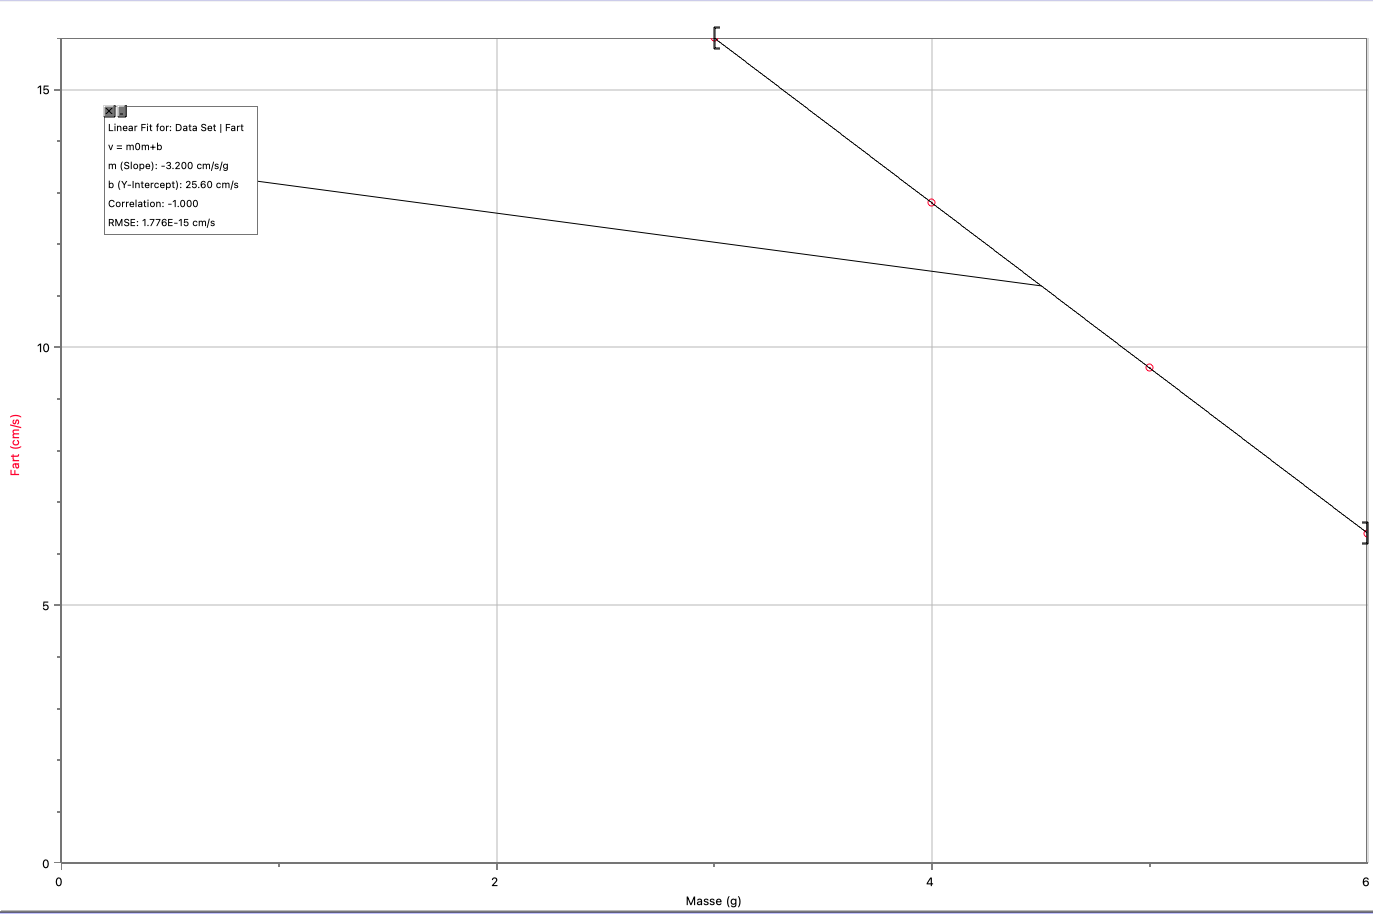
\includegraphics[scale=0.3]{kugle.png}
\end{center}
\caption{Resultaterne afbildet i et koordinatsystem med lineær regression lavet i Logger Pro}
\label{fig:kugle}
\end{figure}
Fra regressionen har vi, at 
\[
v=-3,2 \;\unit{cm/sg} \cdot m + 25,6 \;\unit{cm/s} 
\] 
Derfor gælder der, at
\begin{equation*}
\begin{split}
  v=0 &\implies m=\frac{25,6 \;\unit{cm/s} }{3,2 \;\unit{cm/sg} } = 8,0 \;\unit{g} 
\end{split}
\end{equation*}
Loddet skal altså have en masse på $8,0 \;\unit{g} $, hvis kuglen skal hænge stille. \\[1ex]
\textbf{b.}
Størrelsen af opdriften er bare størrelsen af tyngdekraften på den fortrængte væske.
\begin{equation*}
\begin{split}
  F _{\text{op} }&=V \cdot \rho \cdot g\\
  &=5,6 \;\unit{cm^3} \cdot 1,26 \;\unit{g/cm^3} \cdot 9,8 \;\unit{m/s^2} \\
  &=5,6 \cdot 10^{-6} \;\unit{m^3} \cdot 1,26 \cdot 10^3 \;\unit{kg/m^3} \cdot 9,8 \;\unit{m/s^2} \\
  &\approx 6,9 \cdot 10 ^{-2} \;\unit{N} 
\end{split}
\end{equation*}
Altså er størrelsen af opdriften på kuglen $6,9 \cdot 10 ^{-2}\;\unit{N} $.\\[1ex]
\textbf{c.} 
Når kuglen hænger stille er $F_{\text{gnid} }=0$, og der gælder så (hvor $F _{\text{lod} }$ er tyngdekraften på loddet), at
\begin{equation*}
\begin{split}
  F _{t}=F _{\text{op} }+F _{\text{lod} } &\iff m _{\text{kugle} }=\frac{F _{\text{op} }+m _{\text{lod}}\cdot g}{g}\\
  &\iff m _{\text{kugle} }=V_{\text{kugle}} \cdot \rho _{\text{væske} } + m _{\text{lod} }
\end{split}
\end{equation*}
Vi kan da indsætte de tilhørende værdier og regne massen af kuglen ud.
\begin{equation*}
\begin{split}
  m _{\text{kugle} }&=V_{\text{kugle}} \cdot \rho _{\text{væske} } + m _{\text{lod} }\\
  &=5,6 \;\unit{cm^3} \cdot 1,26 \;\unit{g/cm^3} + 8,0 \;\unit{g} \\
  &=15,056 \;\unit{g} \\
  &\approx 15 \;\unit{g} 
\end{split}
\end{equation*}
Da vi både kender kuglens masse og volumen, kan vi regne dens densitet.
\begin{equation*}
\begin{split}
  \rho _{\text{kugle} }&=\frac{m _{\text{kugle} }}{V _{\text{kugle}}}\\
  &=\frac{15,056 \;\unit{g} }{5,6 \;\unit{cm^3} }\\
  &\approx 2,7 \;\unit{g/cm^3} 
\end{split}
\end{equation*}
Ved opslag i Databog fysik kemi ses det, at aluminiums densitet er $2,6989 \;\unit{g/cm^3} $, hvilket passer med vores udregnede resultat.
Kuglens masse er altså $15 \;\unit{g} $ med en densitet på $2,7 \;\unit{g/cm^3} $, og er nok lavet af aluminium. \\[1ex]
\textbf{d.}
Vi ser først, at 
\[
F _{\text{gnid} }=F_t-F _{\text{lod} } - F _{\text{op} }
\] 
hvor det er åbenlyst, at både $F_t$ og $F _{\text{op} }$ er konstante, da de ikke ændrer sig når massen af loddet gør. 
Fra \textbf{a.} har vi, at
\begin{equation*}
\begin{split}
  v=-3,2 \;\unit{\frac{cm/s}{g}} \cdot m _{\text{lod} } + 25,6 \;\unit{cm/s} &\iff m _{\text{lod} }=\frac{25,6 \;\unit{g\cdot cm/s }-v \;\unit{g}  }{3,2 \;\unit{cm/s} }\\
  &\iff m _{\text{lod} }=8 \;\unit{g} -\frac{v \;\unit{g} }{3,2 \;\unit{cm/s} }\\
  &\iff F_{\text{lod} } =8 \;\unit{g} \cdot 9,82 \;\unit{m/s^2}  -\frac{v \;\unit{g} }{3,2 \;\unit{cm/s} } \cdot 9,82 \;\unit{m/s^2} \\
  &\iff F_{\text{lod} }=78,56 \;\unit{mN} -v \cdot \frac{3,06875 \;\unit{mN} }{\unit{cm/s} }
\end{split}
\end{equation*}
Vi kender allerede $F_{\text{op} }$ fra \textbf{b.}, og kan nu finde et udtryk for $F _{\text{gnid} }$ udtrykt ved $v$. 
\begin{equation*}
\begin{split}
  F _{\text{gnid} }&=F_t- F _{\text{op} }-F _{\text{lod} }\\
  &=9,82 \;\unit{m/s^2} \cdot 15,056 \;\unit{g} - 69,1488 \;\unit{mN} - 78,56 \;\unit{mN}+v \cdot 3,06875 \;\unit{\frac{\unit{mN}}{\unit{cm/s}}}\\
  &=3,06875 \;\unit{\frac{\unit{mN}}{\unit{cm/s}}} \cdot v + 0,14112 \;\unit{mN} 
\end{split}
\end{equation*}
Imidlertid er det andet led så lille, at vi kan se bort fra det.
Vi har da
\[
F _{\text{gnid} }\approx 3,1 \;\unit{\frac{mN}{cm/s}} \cdot v
\] 
Altså har vi, at $F _{\text{gnid} }$ er ligefrem proportional med $v$ med en konstant $K=3,1 \;\unit{\frac{mN}{cm/s}}$, hvilket var, hvad vi ville vise.\\[1ex]
\textbf{e.}
Da der er tale om et kugleformet legeme, der bevæger sig langsom gennem væsken, så må Stokes' lov gælde.
\begin{equation*}
\begin{split}
  F _{\text{gnid} }=K \cdot v=6 \cdot \pi \cdot \eta \cdot r \cdot v &\iff \eta=\frac{K}{6\pi \cdot r}\\
  &\iff \eta =\frac{K}{6\pi \cdot \sqrt[3]{\frac{3V}{4\pi}}}
\end{split}
\end{equation*}
Siden vi både kender $K$ og $V$ kan vi nu direkte beregne viskositeten
\begin{equation*}
\begin{split}
  \eta&=\frac{3,06875 \;\unit{\frac{mN}{cm/s}} }{6\pi \cdot \sqrt[3]{\frac{3 \cdot 5,6 \;\unit{cm^3}}{4 \pi}}}\\
  &\approx 1,5 \;\unit{Pa \cdot s} 
\end{split}
\end{equation*}
hvilket var, hvad vi skulle vise. 
\begin{question}{Haglvejr}{}
  Under et voldsomt haglvejr falder der store hagl, som vist på billedet.
  \begin{itemize}
    \item[a.] Tildel passende værdier til relevante fysiske størrelser, og brug disse til at vurdere den fart, hvormed et af de viste hagl rammer jorden. Gør herunder rede for relevante antagelser.
  \end{itemize}
\end{question}
\sol \\
\textbf{a.}
På billedet ses, at haglkuglernes diameter er halvdelen af længden af langefingeren.
Min langefinger er målt til at have en længde på $8,0 \;\unit{cm} $.
Altså må haglkuglerne have en radius på
\[
r=\frac{1}{2} \cdot \frac{1}{2} \cdot 8,0 \;\unit{cm} =2,0 \;\unit{cm} 
\] 
Da der er tale om en stor kugle gennem luften, så må der være tale om turbulent strømning og $v^2$-loven må gælde.
Når haglet opnår sin terminale fart gælder der
\begin{equation*}
\begin{split}
  F_t=F_{\text{luft} } &\implies m_{\text{hagl} } \cdot g=\frac{1}{2} \cdot c_w \cdot \rho_{\text{luft} }\cdot A \cdot v^2\\
  &\implies v=\sqrt{\frac{2 \cdot m _{\text{hagl} } \cdot g}{c_w \cdot \rho_{\text{luft}}\cdot A }}
\end{split}
\end{equation*}
Vi ved da, at
\begin{equation*}
\begin{split}
  m _{\text{hagl} }&=\rho _{\text{is} }\cdot \frac{4}{3}\pi r^3\\
  A&=\pi \cdot r^2
\end{split}
\end{equation*}
Altså gælder der
\begin{equation*}
\begin{split}
  v&=\sqrt{\frac{2 \cdot \rho _{\text{is} }\cdot \frac{4}{3}\pi r^3 \cdot g}{c_w \cdot \rho_{\text{luft}}\cdot \pi \cdot r^2 }}\\
  &=\sqrt{\frac{8 \cdot \rho _{\text{is} } \cdot r \cdot g}{3 \cdot c_w \cdot \rho_{\text{luft}}}}\\
  &=\sqrt{\frac{8 \cdot 917 \;\unit{kg/m^3} \cdot 2,0 \cdot 10^{-2} \;\unit{m}  \cdot 9,82 \;\unit{m/s^2} }{3 \cdot 0,47 \cdot 1,30 \;\unit{kg/m^3} }}\\
  &\approx 28 \;\unit{m/s} 
\end{split}
\end{equation*}
Farten, hvormed det viste hagl rammer jorden er altså $28 \;\unit{m/s} $.
\end{document}
